\chapter{Introduction}\label{cap.introduccion}

\setlength{\parindent}{0pt}

%As engineers we want to build systems that are better than our brain, like the entity of figure \ref{introsss}, it has 100 billion computing elements, it solves problems not soluble by previous machines, and it only requires 20 watts of power, indeed we are referring to the brain of the person standing in front of the computer.
%
%\begin{figure}[H]
%\centering         
%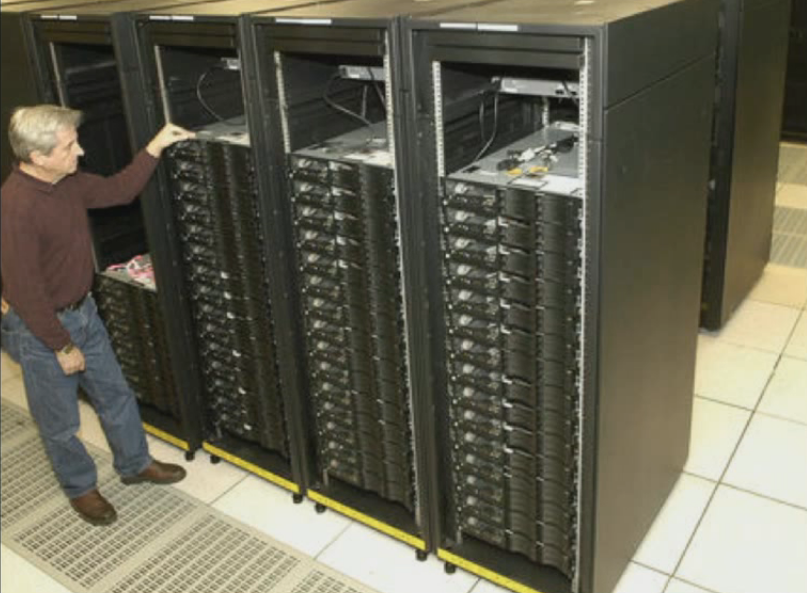
\includegraphics[width=7cm]{intro2/computer.png}
%\caption{Computing machines.} \label{introsss}
%\end{figure}

As engineers we want to build systems that are better than our brain, to point out the difficulty of this endeavor, we can summarize the brain characteristics as follows: it has 100 billion computing elements, processing and memory are performed by the same components, works as parallel recurrent paradigm, it solves problems not soluble by previous machines, and it only requires 20 watts of power.


There are several computation challenges very interesting but, despite recent success in most of them, it struggles us to reach brain performance and efficiency. Machines have beaten us in extracting information for large collection of data, they can process larger amount of data than the humans. Also, in memory, they beat us, they can store more information and access faster than humans. It is not a matter of speed computation, they also exceed us in reasoning tasks, like playing chess or Go. However, in low-level sensorimotor skills, like seeing or walking our brains performs better than machines. These kinds of tasks, that humans perform unconsciously, for a computer is really complex to achieve it.

This fact is called the Moravec's paradox, this paradox came out during the dawn of Artificial Intelligence back in the 80s when M.Minsky, R.Brooks, and H. Moravec tried to mimic human skills by reverse engineer the brain. This paradox consists in, contrary to traditional assumptions, high-level reasoning requires very little computation, but tasks involving with  perception, attention, visualization, motor, and social skills require enormous computational resources and are difficult to transfer to machines.

One possible explanation of this paradox, is based on evolution, humans skills are implemented biologically, improvement over years of natural selection. The older a skill is, the more time natural selection has had to improve the design. In contrast, abstract thought developed only very recently is easy to implement due this shorter developed.

These categories of intelligence will take much more time to implement in machines, but research keep going.

\section{Computer vision}


In the late 60s, computer vision began at universities that were pioneering artificial intelligence. It was meant to mimic the human visual system, as a stepping stone to endowing robots with intelligent behaviour. In 1966, it was believed that this could be achieved through a summer project, by attaching a camera to a computer and having it \textit{describe what it saw}.

This describes the excitement of that time and their underestimation of the field as we stated in the previous section. Although, it is a complex area of studying, it has been a lot of developments during fifty years, real world application have been developed and are part of daily use. 

One recent application of computer vision, is the usage of these technique on robotics, in particular on autonomous cars. These cars developed by technological giants are being used in some States of US. In these systems, the surrounding information is extracted by cameras. As we can observe in figure \ref{intro1} are used to detect other types of vehicles on the road.

\begin{figure}[H]
\centering         
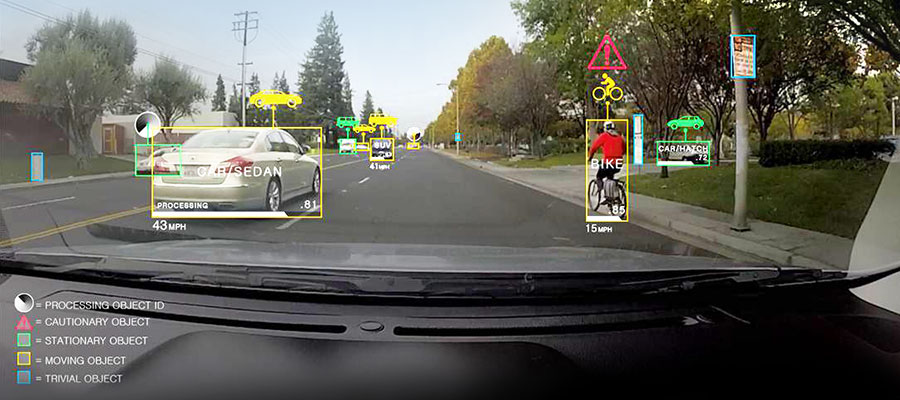
\includegraphics[width=8cm]{aplicaciones/autonomous.jpg}
\caption{Frontal view of autonomous car.} \label{intro1}
\end{figure}



Another computer vision's area is medical imaging, this area studies the techniques and process of creating visual representations of the interior of a body for clinical analysis. One example is the tractography map, like the one in figure \ref{introTractog} created from a diffusion weighted images, it allows us to establish connections between different areas of the brain.

\begin{figure}[H]
\centering         
\includegraphics[width=8cm]{aplicaciones/diffusion.jpg}
\caption{Tractography map.} \label{introTractog}
\end{figure}


One pioneer in technology is the automation industry, technology used to manufacture quickly and better. Computer vision is deeply used in factories, their usage is for inspection quality of manufactured products, they can check whether a product fulfill quality characteristics, as we can observe in figure \ref{introFactory}.

\begin{figure}[H]
\centering         
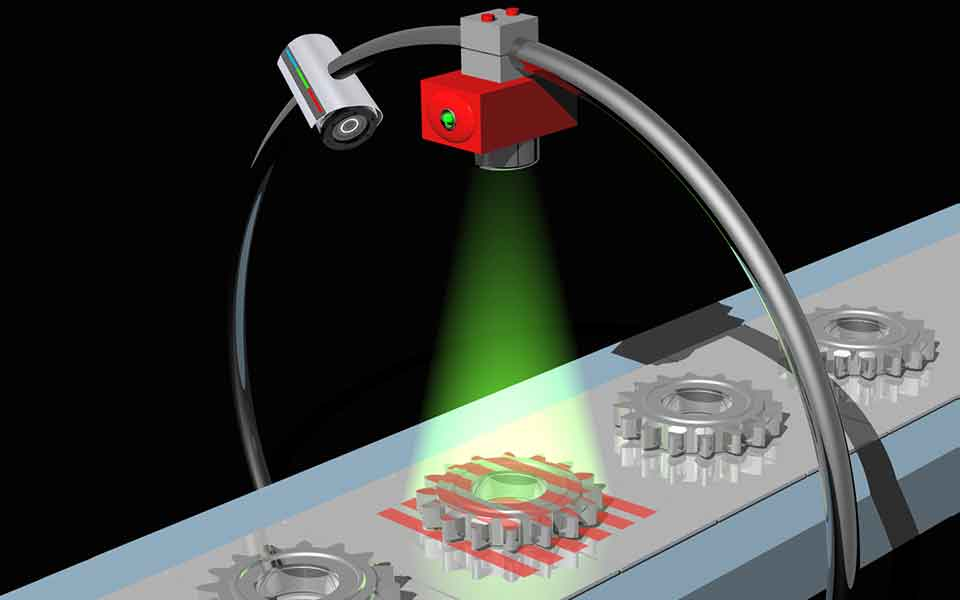
\includegraphics[width=8cm]{aplicaciones/factory.jpg}
\caption{Camera for inspection.} \label{introFactory}
\end{figure}

%
%Another application of computer vision is to get , in these types of application cameras can work by itself, but it has better results when it is combined with depth sensors. This is called RGBD sensor, it allows to estimate the depth of the scene and superimpose the texture, as we can observe in figure \ref{introrgbd}

Finally, another application of computer vision, is to mix the information provided by the camera with graphics, this is called, augmented reality. One example of it, is the work of the company Snapchat, it allows you to render different artifacts on an image and share it with your friends. We can observe one example on figure \ref{introrgbd}.

\begin{figure}[H]
\centering         
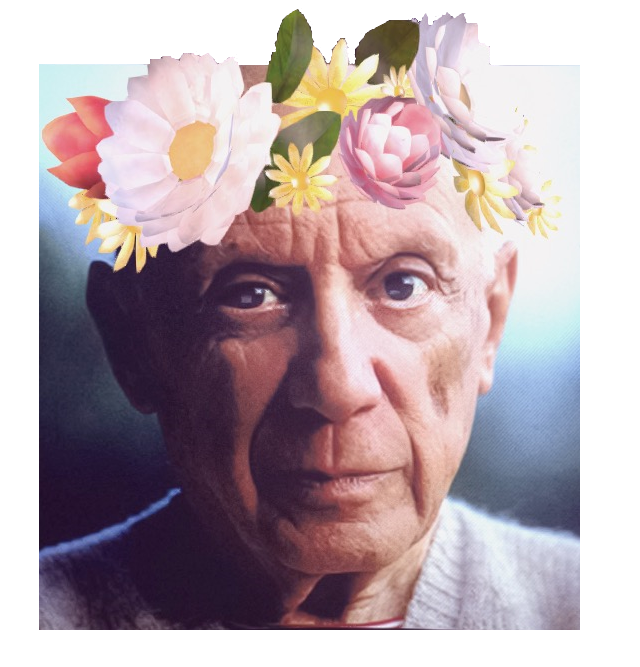
\includegraphics[width=8cm]{aplicaciones/picassioHuai.png}
\caption{Augmented reality image.} \label{introrgbd}
\end{figure}





\section{Object tracking}

In the widely computer vision field there are several study areas, one of them is Object tracking. It consists in estimating target state over time from image sequences. As a state we can embedded the position, velocity, shape, appearance or any interesting characteristics. It is very challenging field due to:


\begin{itemize}

\item Variations due to geometric changes, some targets might be deformed as they move in the scene which would change their structure.

\item Variations due to photometric factors, the appearance of the targets might change due to changes in illumination.

\item Occlusions, targets might mix with other elements of the scene from the camera perspective.

\item Image quality, the image sequences could incorporate noise or a low resolution.

\item Similar objects in the scene, this could cause problems to maintain the identity of targets.

\end{itemize}

To solve these problems the community has used the following paradigms \cite{visualTrackingSurvey}:

\begin{itemize}

\item \textbf{Tracking using matching}, these kind of methods performs a matching of the representation between the current and the possible candidates in the next frame. Key points of these methods are the representation and the the similarity measurement to perform the matching. The most famous methods are Normalized Cross-Correlation \cite{trackNcc}, Lucas-Kanade tracker \cite{klt}, Kalman appearance tracker \cite{kalmm} and Mean shift tracking  \cite{meanshift}. 

\item \textbf{Tracking-by-detection}, these kinds of methods build a classifier to distinguish target pixels from the background. Once you have the detection, you need a data association method to link those detections. Traditionally the community has used kernel methods with support vector machines \cite{struc} to perform the detections, but in the recent years people are shifting to neural networks. In the data association algorithms graph theory techniques are dominant \cite{dataAsso1} \cite{dataAsso2}.


\item \textbf{Tracking learning and detection}, this is an extension of the previous category. It includes a mechanism to update the classifier during the execution of the system. This learning procedure allows the algorithm to be invariant to changes in the target. The most famous s algorithms are the Predator \cite{tld} and the Alien \cite{alien}.



\end{itemize}


These kinds of algorithms are quite mature and are deployed in real life applications. Like all the informatics process it allows us to process a huge quantity of information really quickly.

In video surveillance, it allows us to track all the targets without human intervention and notify when there are dangerous situations. 

\begin{figure}[H]
\centering         
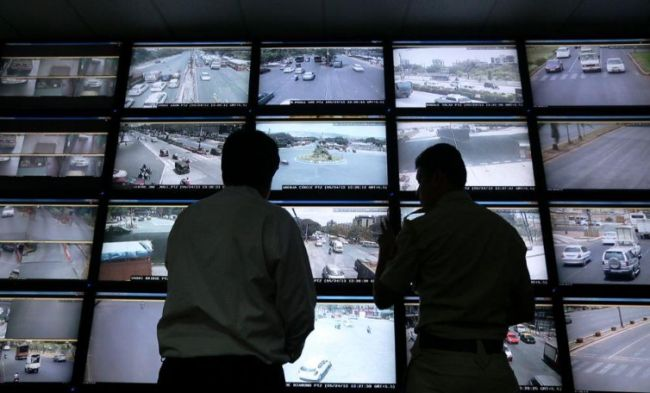
\includegraphics[width=8cm]{aplicaciones/policias.jpg}
\caption{Control room.} \label{introTracking1}
\end{figure}


For science, it allows us to study the environment, in the case of the figure \ref{introTracking2}, for humans it will be difficult to do not miss the correct identity of these ants. With information supplied by the tracking, scientist can study how animals move and interact with others.

\begin{figure}[H]
\centering         
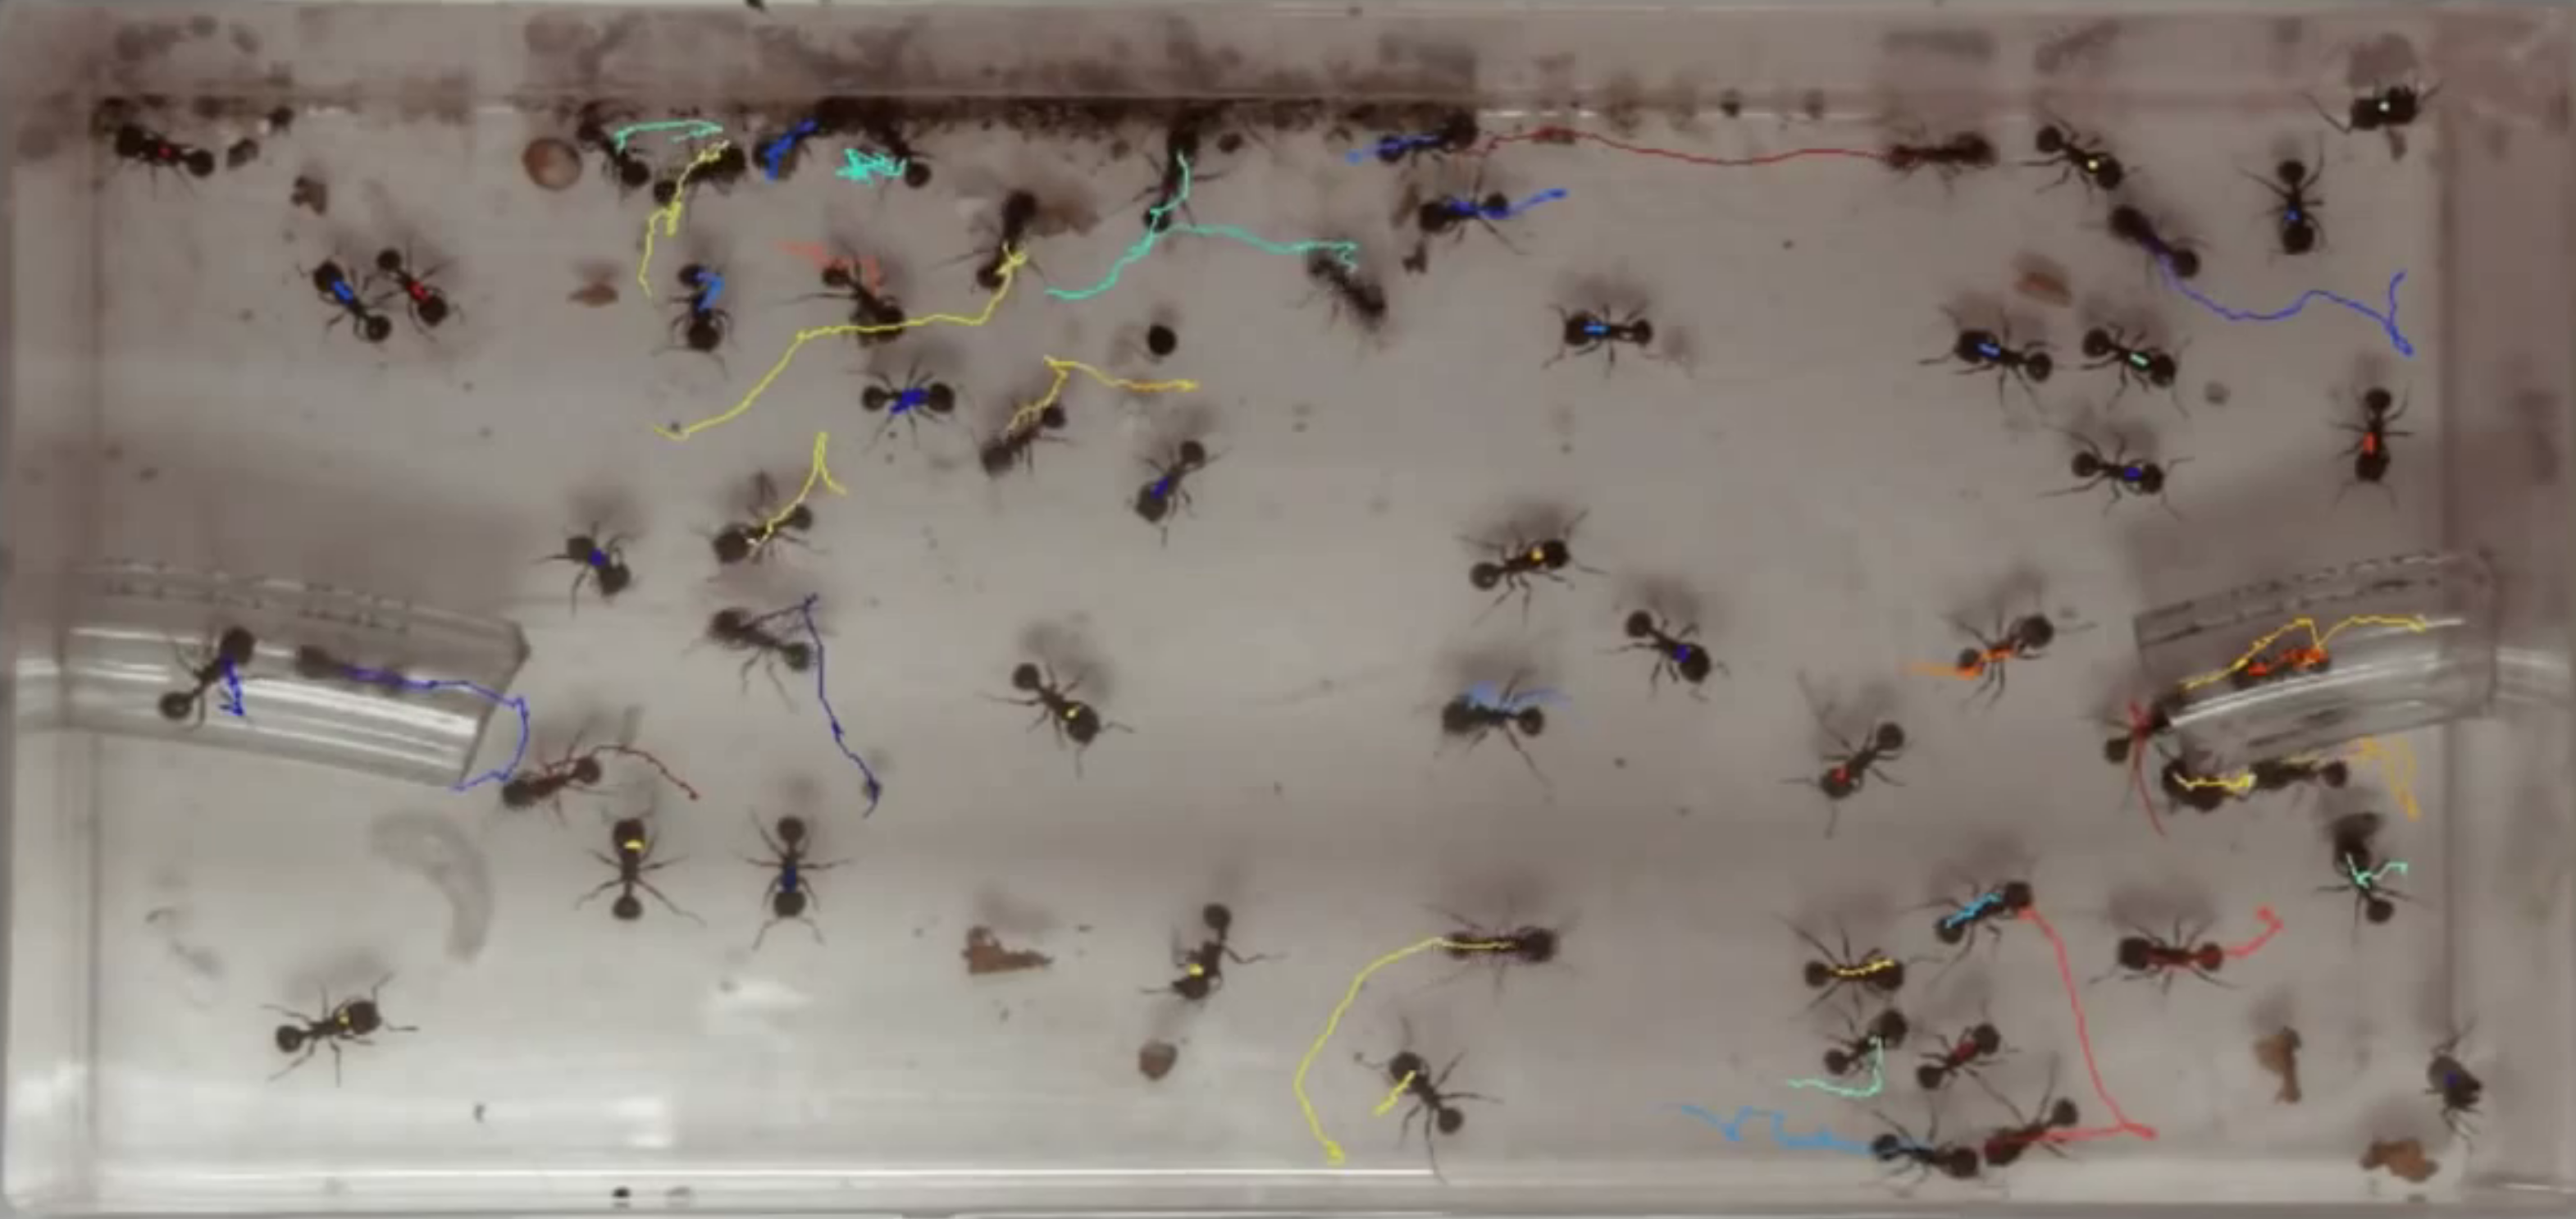
\includegraphics[width=8cm]{aplicaciones/Seleccio_007.png}
\caption{Visual tracking for science.} \label{introTracking2}
\end{figure}

These algorithms are deeply used in all kind of sports like the NBA and NFL. In this situations the algorithm tracks the players during the game and allows to analysis his performance and the strategy of the team, like in figure \ref{introTracking3} .

\begin{figure}[H]
	
\centering

\subfigure[Input image]{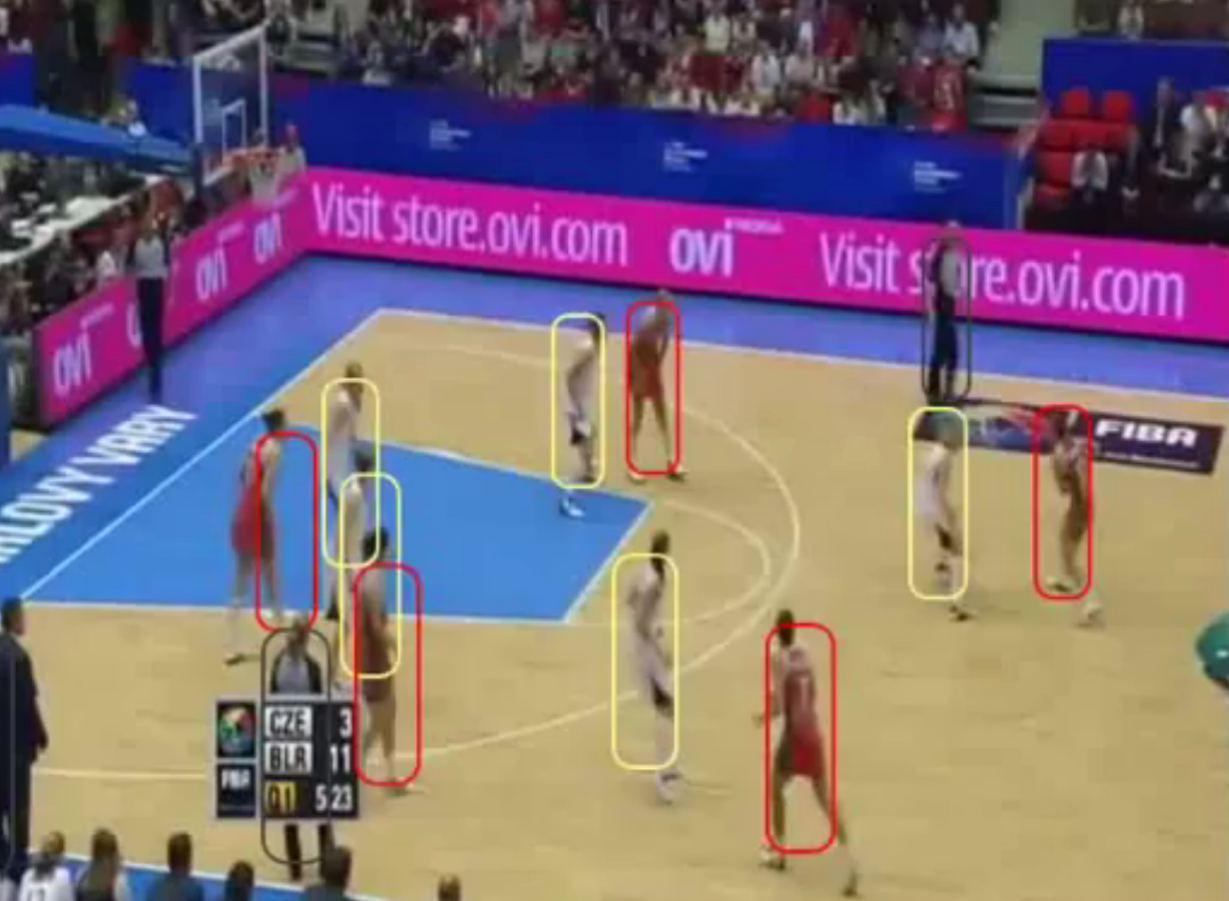
\includegraphics[width=5cm]{aplicaciones/Seleccio_010.png}}
\subfigure[Layout ]{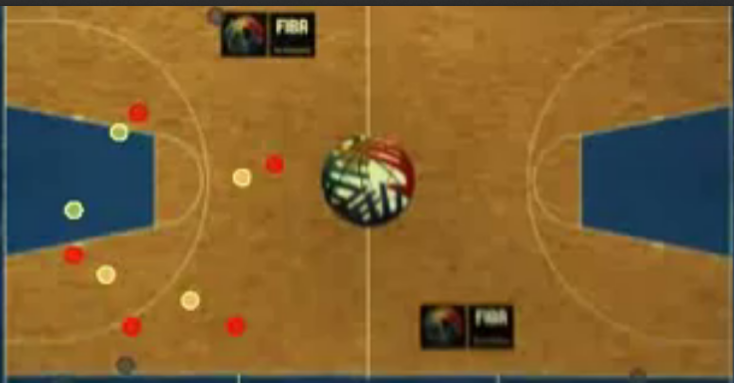
\includegraphics[width=7cm]{aplicaciones/Seleccio_011.png}}\\


\caption{Visual tracking for sports analysis.}
\label{introTracking3}
\end{figure}

In artistic performance, these algorithms are used to track the subject and render some graphics in the scene, like an extension to video of augmented reality. In the example of the figure \ref{introTracking4}, the systems tracks the singer's head and projects a visualization of his voice.

\begin{figure}[H]
\centering         
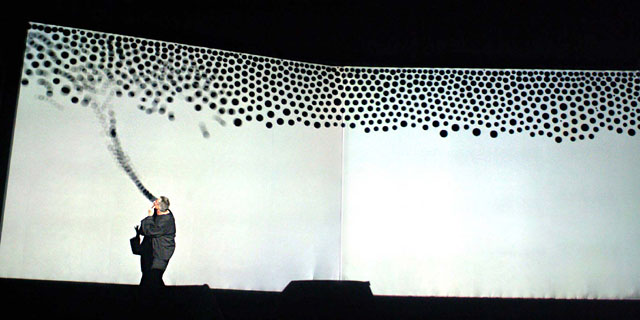
\includegraphics[width=12cm]{aplicaciones/singing.jpg}
\caption{Visual tracking for art.} \label{introTracking4}
\end{figure}


\section{Deep learning in computer vision}

Deep learning has raised by drastic improvements over reigning approaches towards the hardest problems in Artificial intelligence (AI), massive investments from industry giants, and exponential growth in research publications. Deep learning is a tool inside the machine learning toolbox, the goal is to make machines learn.

The first incursion was made by Frank Rosenblatt, the Percetron \cite{rosenblat}. Rosenblatt conceived of the Percetron as a simplified mathematical model of how the neurons in our brains operate. This model of the neuron built on the work of McCuloch-Pitts \cite{McCulloch}, who showed that a neuron model could model the basis OR/AND/NOT functions. Which in the early days of Artificial intelligence was great, because the predominant thought at that time was that making computers able to perform formal logical reasoning would essentially solve AI. However, the McCuloch-Pitts model lacked a mechanism for learning, which was crucial for it to be usable for AI. This is were the Perceptron exceeded, Rosenblatt came up with a way to make such artificial neurons learn, inspired by the Hebb's Rule. This learning method was as follows: if the output of the perceptron was low, increase the weights, otherwise decrease the weights if the output is too high. Also, another researchers came with ADALINE \cite{adaline} learning procedure, they used the signal before the activation function to compute the derivative, how much the error changes when each weight is changed can be used to drive the error down and find the optimal weights values. Similar as we train the networks nowadays.

Researchers were really excited about this idea of Connectionism: that networks of such simple computational units could be vastly much more powerful and solve the hard problems of AI. But in 1969, Minsky and Papert  published an analysis on the limitations of perceptrons \cite{minsky69perceptrons}. The biggest criticism was that a perceptron could not learn the simple boolean function XOR because it is not linearly separable. However, they stated that it could be learnt with multiple layers perceptron but the learning procedure did not work for multiple layers. After this book, the interest on Neural networks decreased, and initialize a period called \textit{AI winter}, AI shifted to logic programming and common sense reasoning.

This period lasted till 1986 when Rummelhart, Hinton, and Williams published the algorithm of backpropagation \cite{Rumelhart}, which specifically addressed the problems discussed by Minsky in Perceptrons, a method to train multiple layer neural nets. With this discovery in 1989, LeCun showed a real world application, recognized handwritten digits \cite{lecunZip}. The architecture of this model was a convolutional neural network. It was inspired by the Neurocognitron \cite{Fukushima} of Fukushima, which took ideas from studies of the brain. In particular the studies of Hubel and Wiesel, they propose that the visual cortex is formed by a hierarchical model, primarily for simple cells who respond for simple structures and then complex cells respond to a more complicated feature. As we can observe in figure \ref{intro1}, in the lower layer, the network learns Gabor like features, and while going upwards, the networks learns more abstract concepts.




\begin{figure}[H]
\centering         
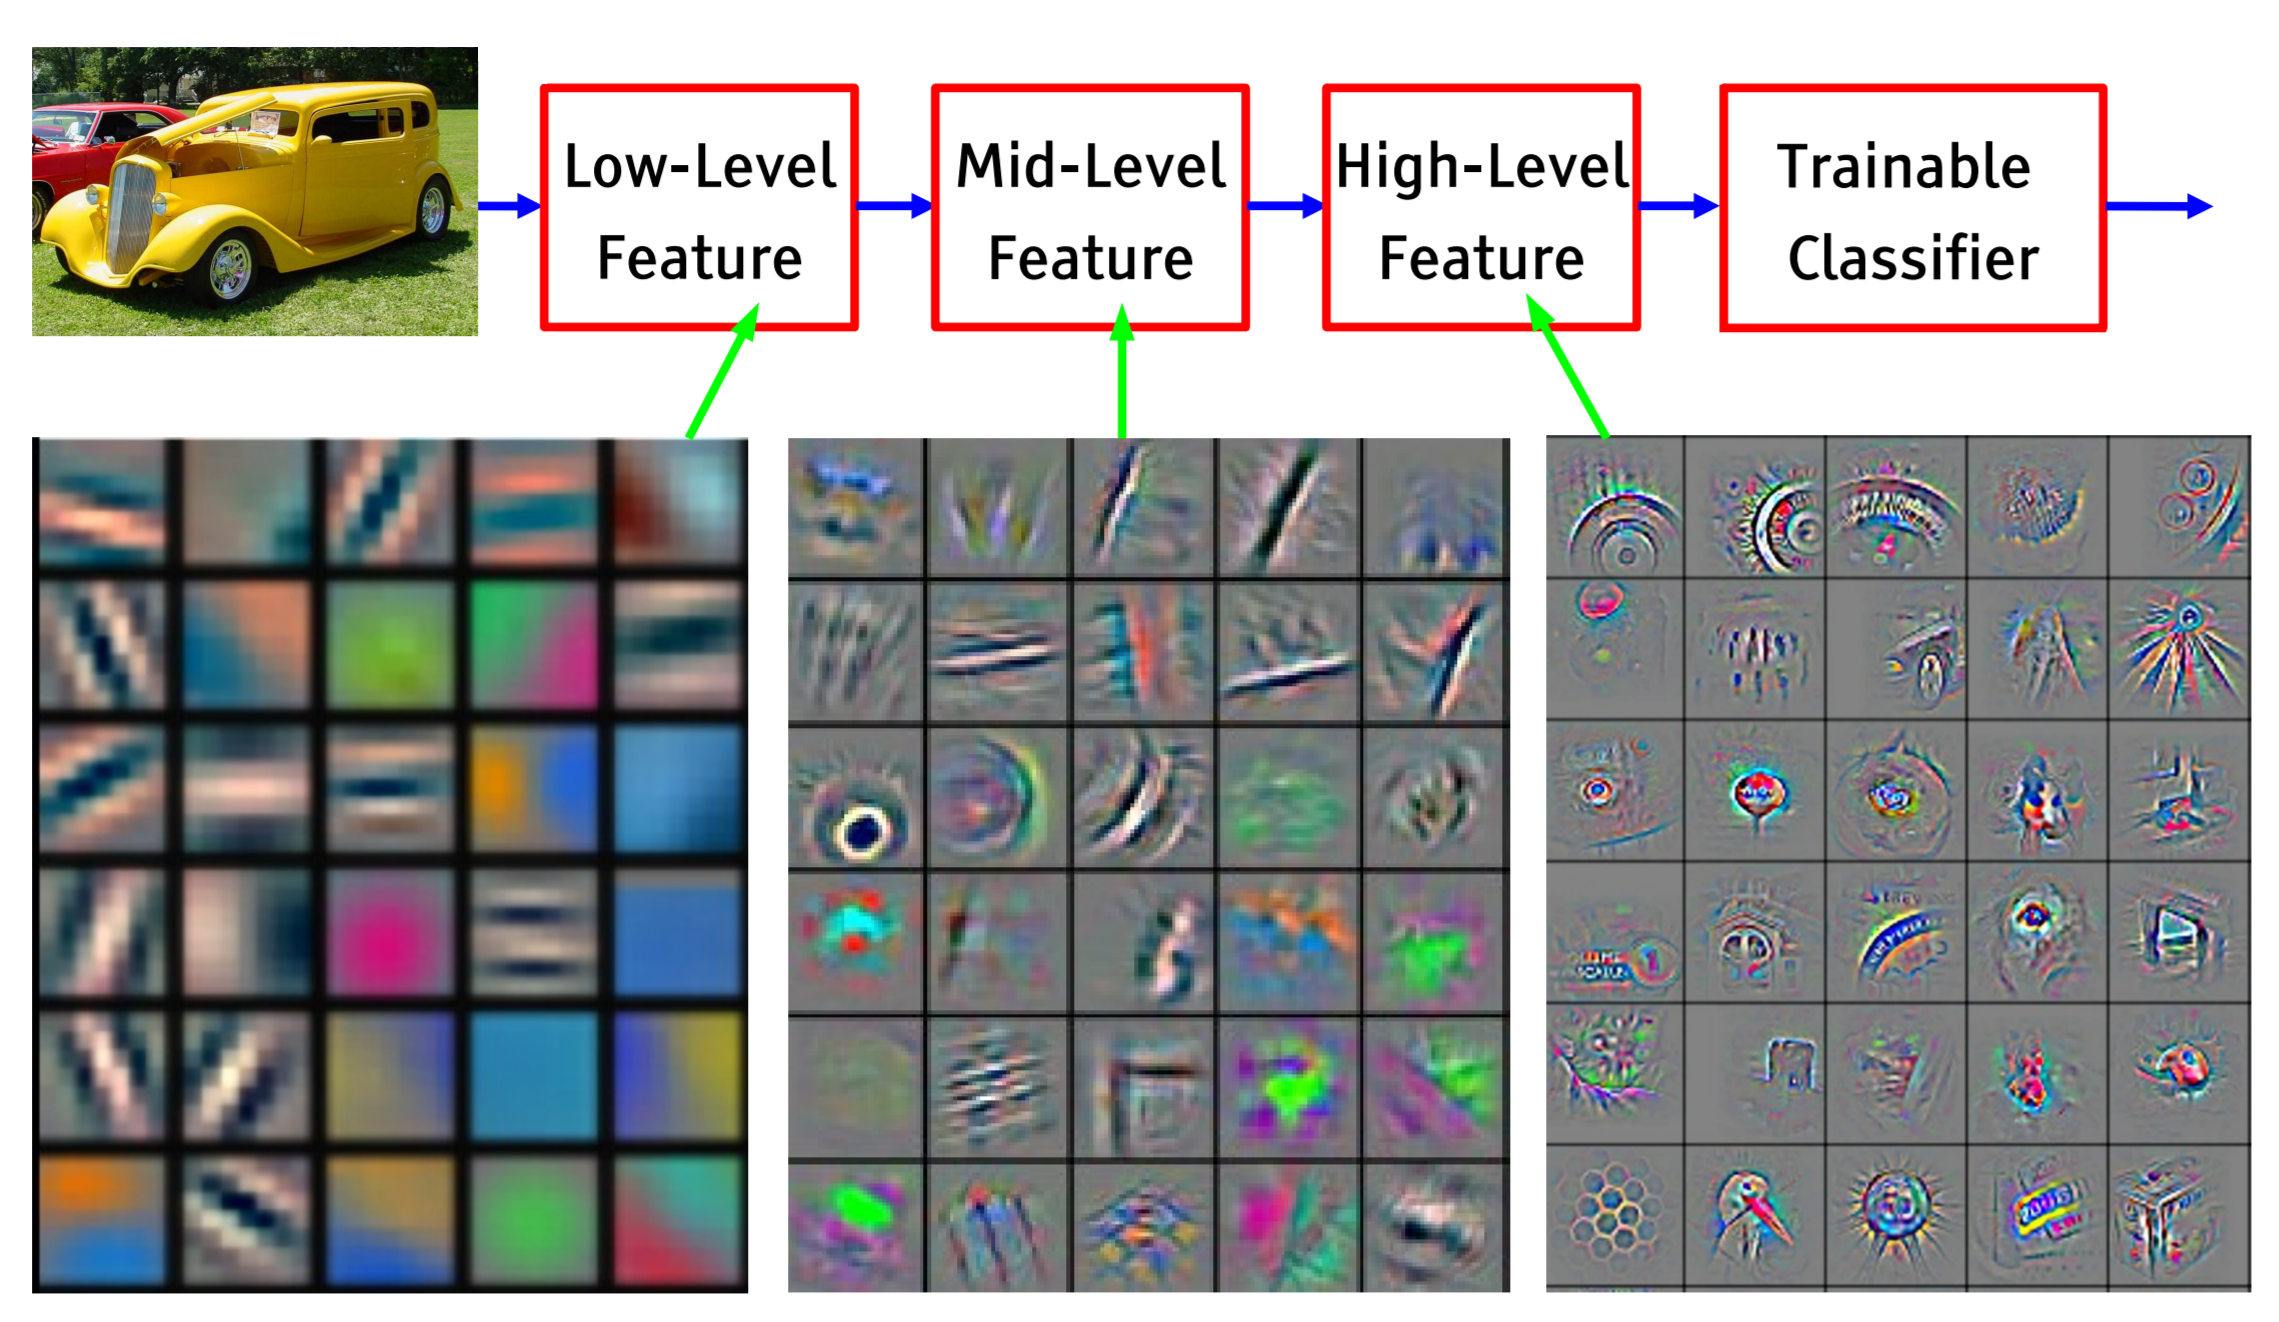
\includegraphics[width=12cm]{intro/model.png}
\caption{Representation of a Convolutional neural network.} \label{intro1}
\end{figure}



But this approach did not scale to larger problems, the biggest source of problems was the vanishing gradients problem. When the backpropagation gradients backpropagates trough the network, in some nodes the local gradient is very low ( in the extreme of the sigmoid functions ) the signal vanishes or saturates. By the 90s other techniques became the method of choice, like support vector machine (SVM). Although some progress was made for other kinds of problems.

\begin{itemize}

\item Unsupervised learning. This type of architectures is used to find a smaller representation of some data from which the original data can be reconstructed, it is useful for compression, visualization, and classification. One example of this architecture with neural networks is the Restricted Boltzmann machine \cite{boltzmann}, developed by Hinton.
%in this setting the neurons behave according to a probability distribution, and form a graphical model. The neuron are hidden %layers, and it can be used to infer information from it.
 
\item Reinforcement learning. The goal of this type of learning is to learn how to make good decisions, it requires rewards, not labels. One example of this sort of systems, is the TD-Gammon \cite{Gammon}, a neural network that learned to be a backgammon player.

%\item Robotics. This was another field separate from Machine Learning where neural nets were very useful. A major example of early neural net use for robotics came from CMU's NavLab in 1989. the neural net learned to control the vehicle using steering data recorded while a human drove \cite{alvin}.

\item Recurrent neural networks. Plain neural networks could not process sequences due to they do not have memory, they need mechanism to remember the pasts outputs. With memory, it can process sequences like audio or text. One approach to this, by Waibel \cite{Waibel} in 1989. 


\end{itemize}


In 2006, there was a breakthrough \cite{hinton06}, Hinton realized that a neural network with many layers really could be trained well, if the weights are initialized in a clever way. The basic idea was to train each layer one by one with unsupervised training ( like an autoencoder architecture ) and finally stack all together and train it in a supervised way. 

Although, these improvements, the big step forward came in 2012, when AlexNet \cite{alexnet} beat the state of the art in the ImageNet challenge, an image classification challenge, where the error rate was $15.3 \%$ whereas the winner of the previous year was $26.3 \%$. In the figure \ref{intro2} we can observe the advance in the state of the art of the ImageNet challenge with the inclusion of deep learning techniques.




\begin{figure}[H]
\centering         
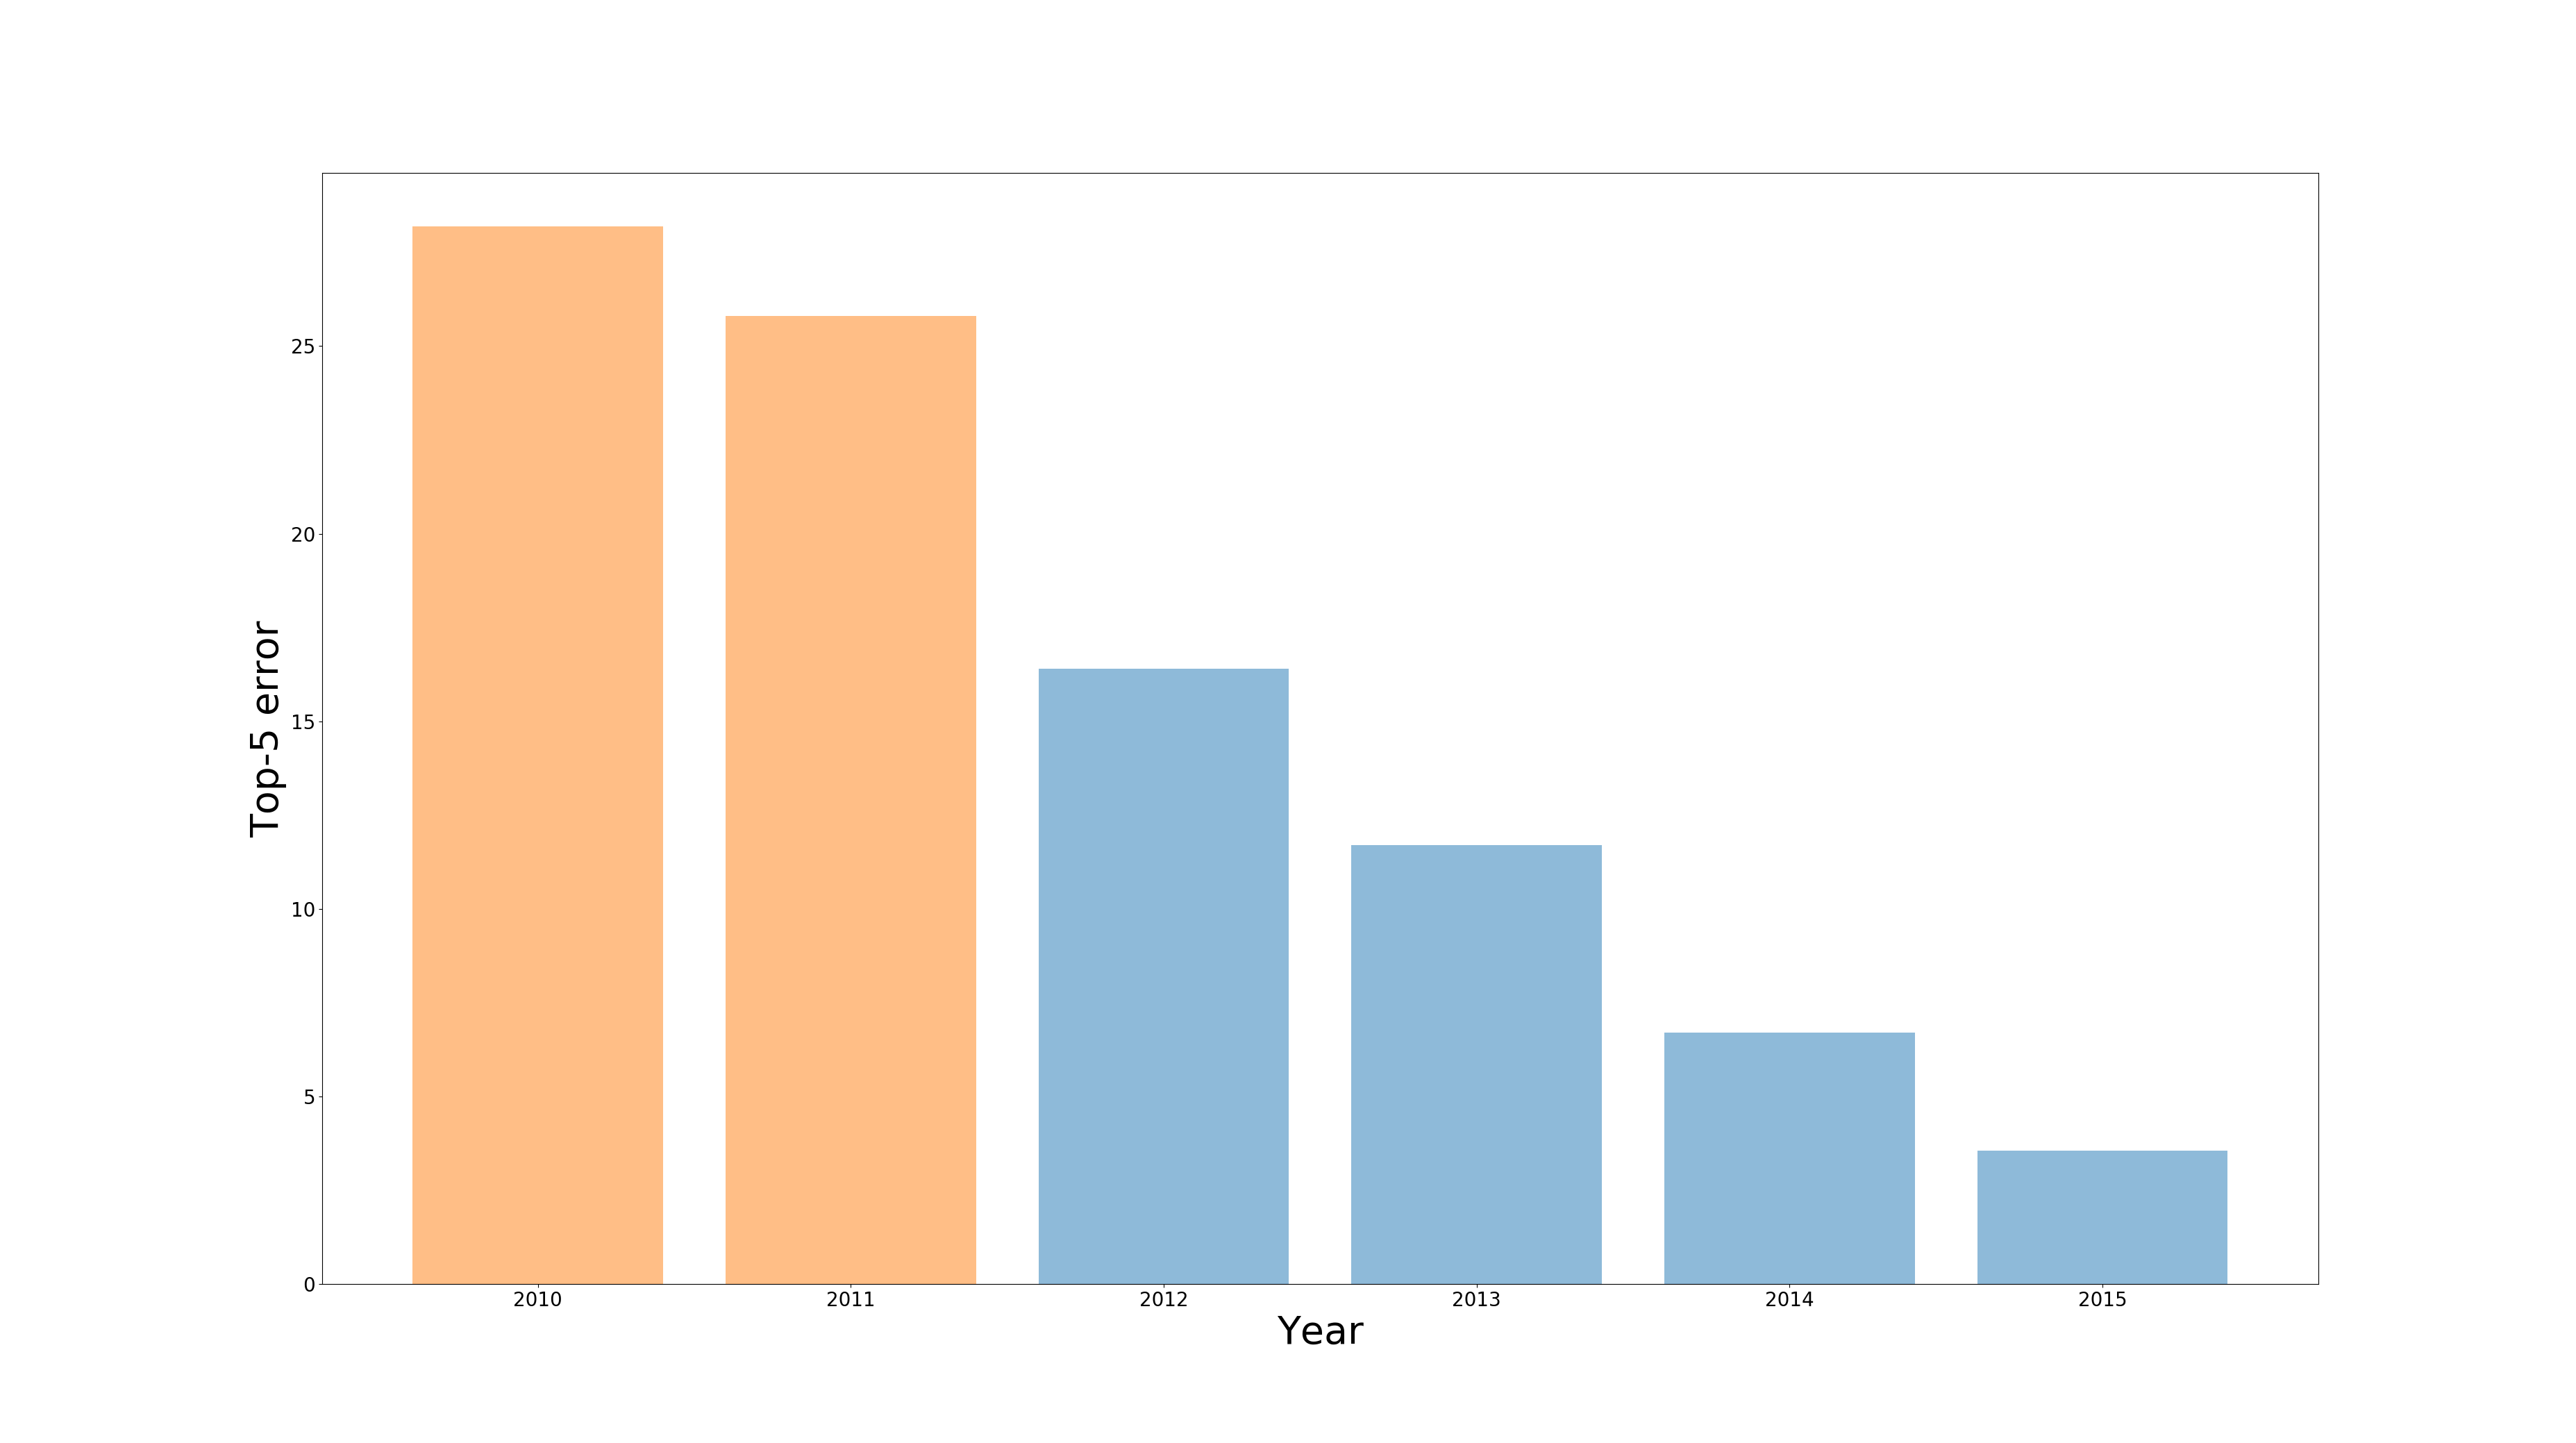
\includegraphics[width=0.7\linewidth]{intro/iamgeWihtou.png}
\caption{Classification error in ImageNet challenge.} \label{intro2}
\end{figure}



The emergence of these techniques were the culmination of decades of research but the step forward was due by three aspects:

\begin{itemize}

\item \textbf{Appearance of large and high quality dataset}, The increasing size and quality of the dataset helps the networks to converge easily.

\item \textbf{Parallel computation}, The increasing of computing capabilities helped train larger models in less time.

\item \textbf{Optimization details}. With the discovery of the proper initialization and activation functions larger networks can be trained.


\end{itemize}












